% REP001 探索：ルールベース3手法の動作と評価（親：W001。問いは未確定）
% コンパイル：uplatex を2回 → dvipdfmx（TEXINPUTS で .claude/templates/progress_report// を参照）
\documentclass[twocolumn, 10pt]{ujarticle}
\usepackage{progress_report}

\begin{document}

\reportid{REP001}
\questionid{W001}
\exploration{既存のルールベース入札手法は，この環境でどう動くか}
\reportdate{20261007}
\summary{%
最終的には新しい入札方法を提案したいが，その前に，既存のルールベース手法（PID，ABid，Online LP）をこのシミュレータで動かすと何が起きるかを確認した。
広告主48社の位置×4エピソードで3手法を比べ，6位置で主要パラメータを振ったところ，全270回が完走し，Online LPのスコア合計がPIDの1.92倍，ABidの1.49倍で最大であった（「Online LPが最良」は論文と一致。PIDとABidの順序は論文と異なる）。
1回の評価は約150〜215秒・約2.5GBで，結果は再現した。ここから，Online LPの優位が報酬の大きさとCPA制約の守り方のどちらに由来するかを知りたい，という問いが生まれた。
}
\beginverification

% ============================================================
\section{目的}\label{sec:e-purpose}
% ============================================================

既存のルールベース入札手法（PID，ABid，Online LP）が，このシミュレータでどう動くかを知る。

% ============================================================
\section{実験}\label{sec:e-exp}
% ============================================================

\subsection{対象のアルゴリズム}\label{sec:e-algo}

3手法とも，各ティックの頭に，そのティックの広告機会（PV）ごとの入札額を「$\alpha\times$価値」の形で決める
（価値は購入確率。ABidだけ価値の2乗を使う）。手法の違いは，入札係数$\alpha$の決め方である。
\begin{itemize}[leftmargin=1.2em, itemsep=0pt, topsep=2pt]
\item \textbf{PID}：予算の使うペースで$\alpha$を上げ下げする。最初は$\alpha=15$。
  毎ティック $x=$（前のティックの支払い$\times$残りティック数）$\div$残り予算 を計算し，
  $x<0.7$なら$\alpha$を1.2倍，$x>1.1$なら0.7倍にする。CPA制約は使わない。
\item \textbf{ABid}：予算も履歴も見ない。入札額$=$CPA制約$\times$価値$\times$（価値$\div$そのティックの価値の平均）。
  価値が平均より高いPVほど強気に入札する。全体の倍率（\texttt{bid\_scale}）は既定で1。
\item \textbf{Online LP}：過去の1日の記録から作った早見表を引く。表は，購入1件あたりの値段が安いPVから順に
  買ったときの，支払いの累計である。今の残り予算で買える範囲の境目の値段を$\alpha$にする
  （上限はCPA制約の1.5倍）。残り予算が多いほど$\alpha$は大きくなる。
\end{itemize}

% 2段抜きの図は，2ページ目の上に出すためにここで宣言する
\begin{figure*}[t]
\centering
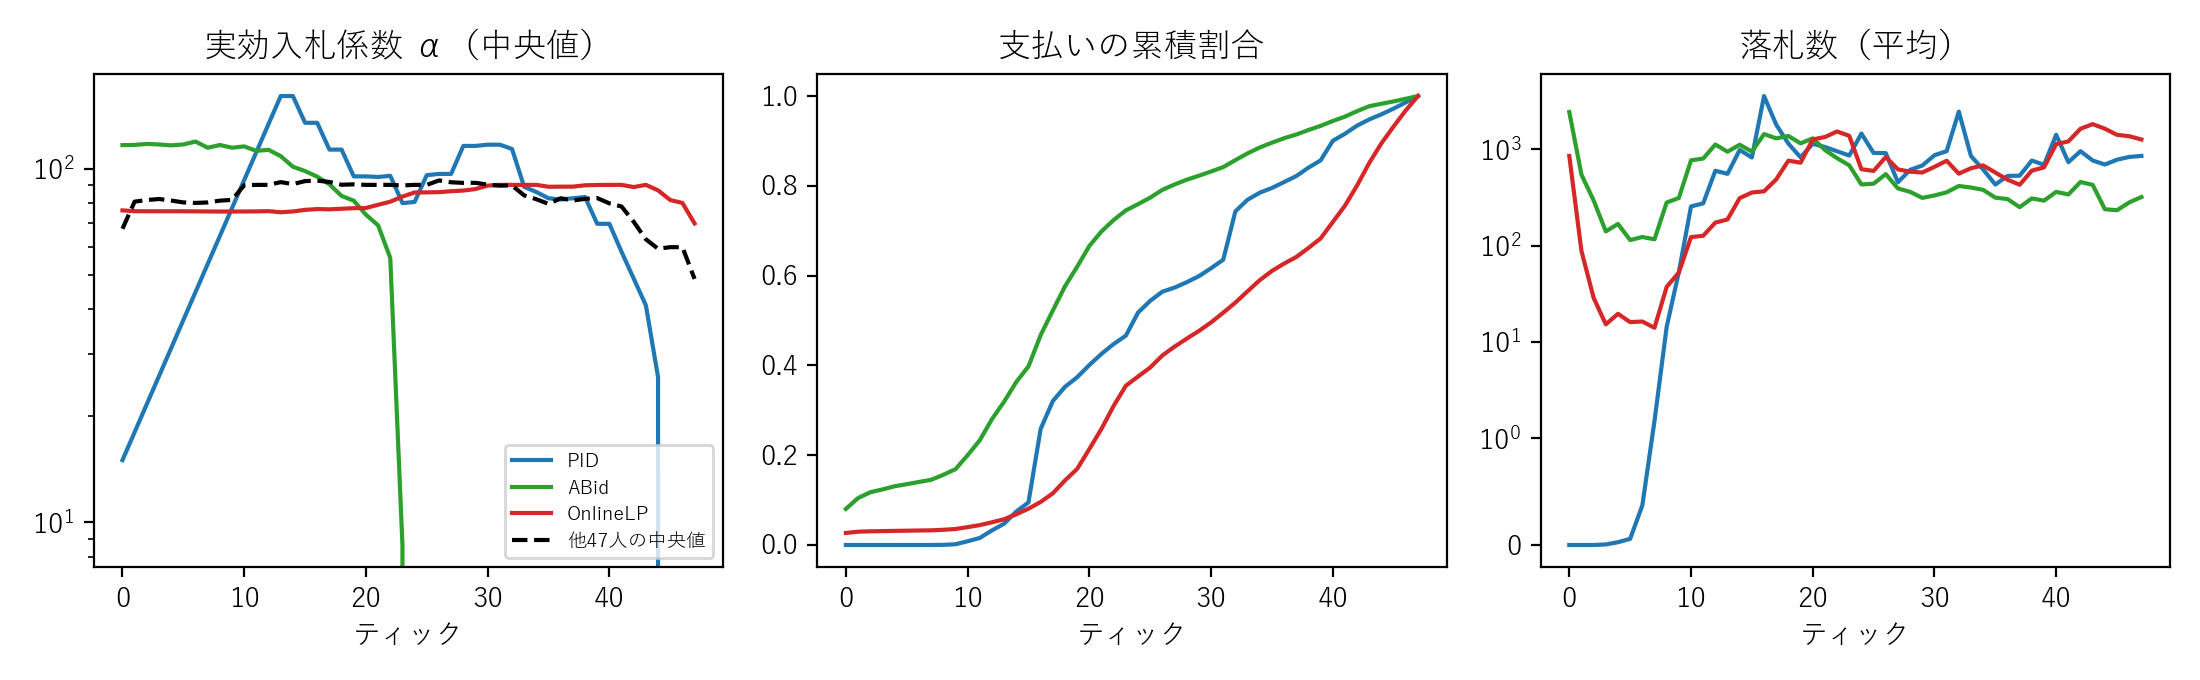
\includegraphics[width=0.8\textwidth]{fig/fig_alpha_time.png}
\caption{既定設定の3手法の時系列（192セルの中央値または平均）。左：実効入札係数$\alpha$（対数軸），中：支払いの累積割合，右：落札数}
\label{fig:alpha}
\end{figure*}
\begin{figure*}[t]
\centering
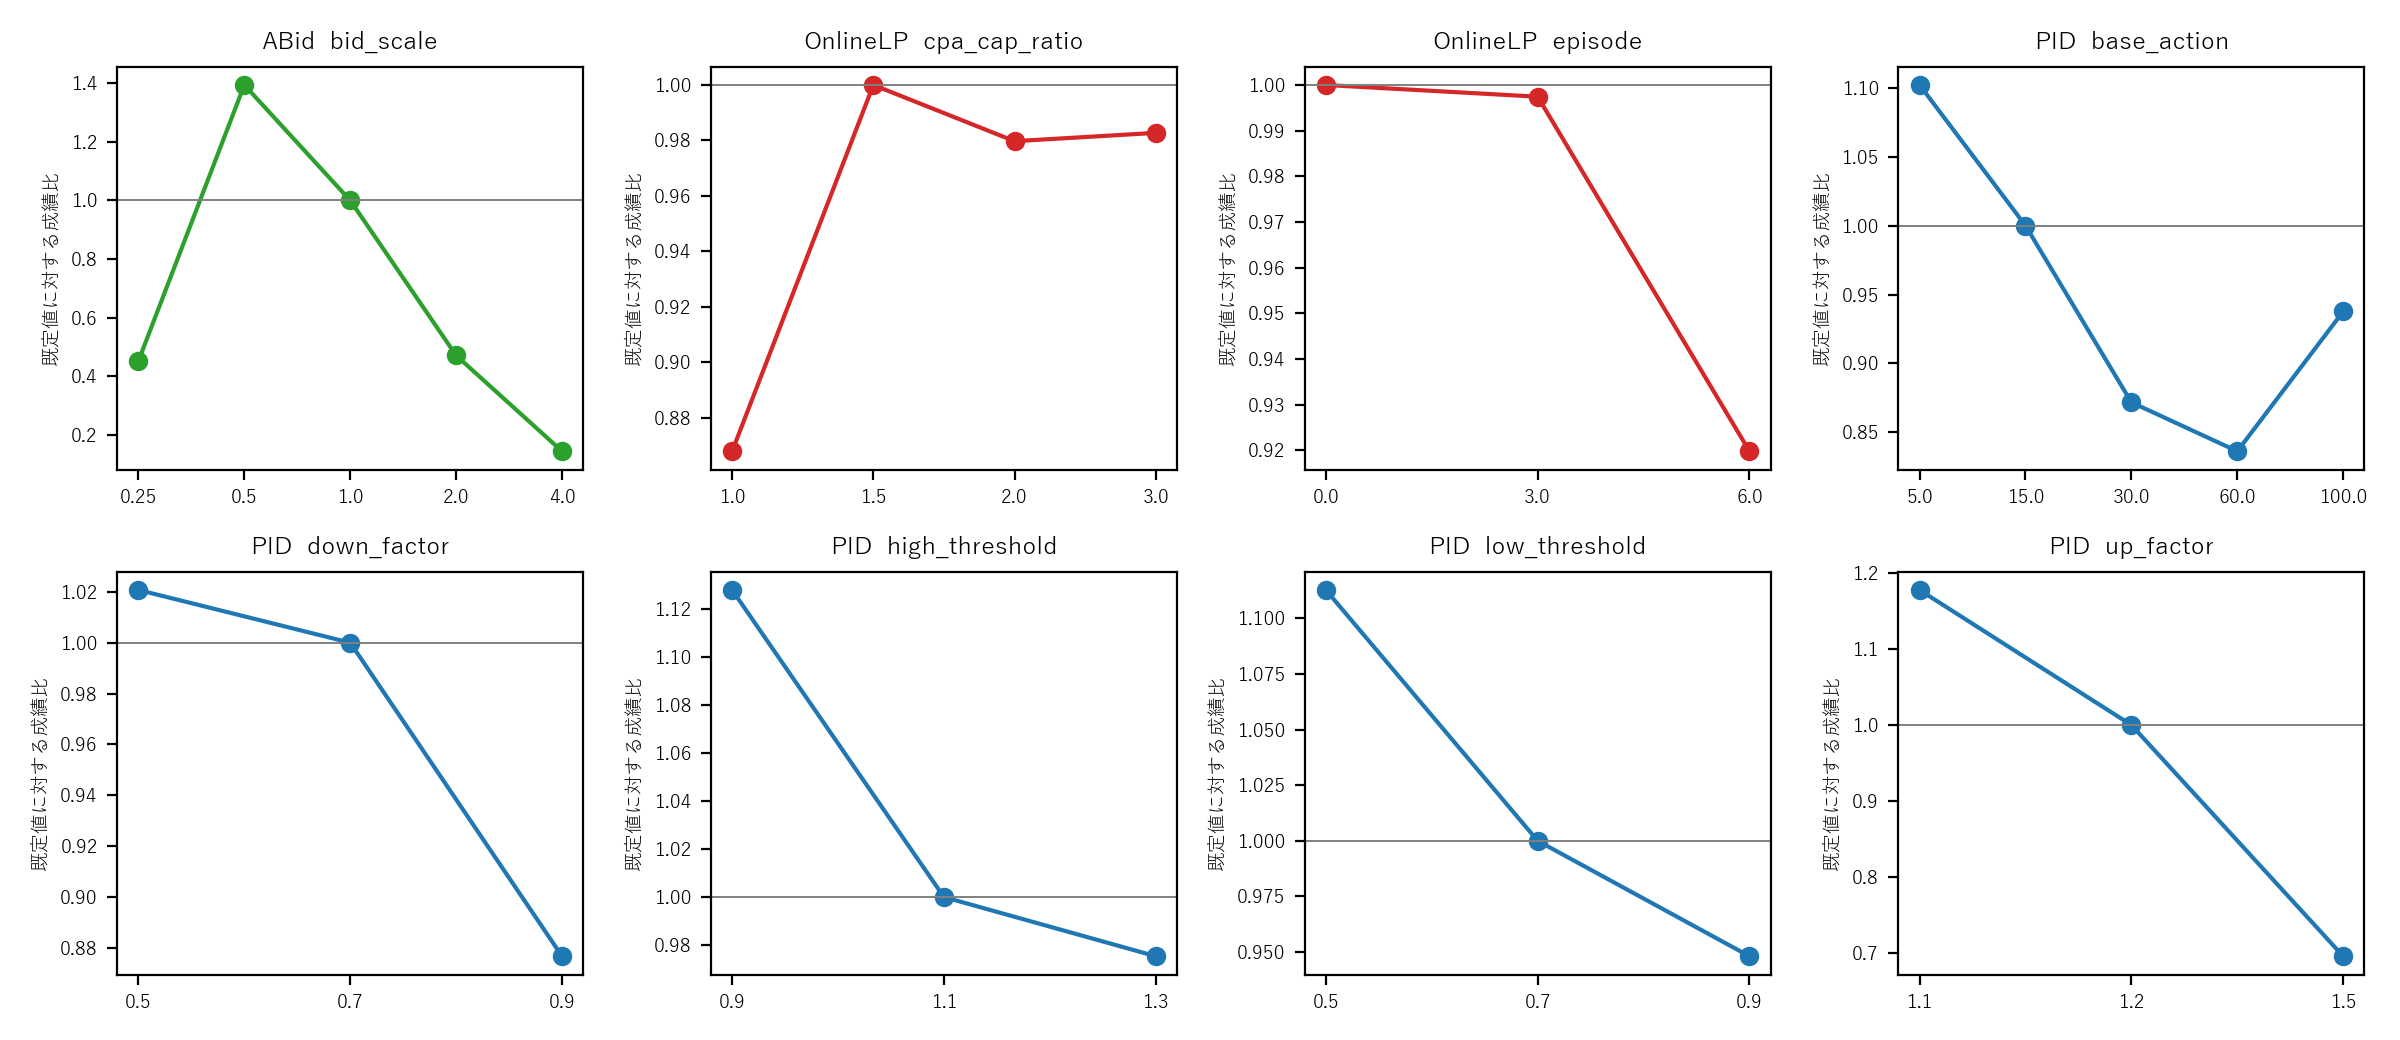
\includegraphics[width=0.8\textwidth]{fig/fig_sweeps.png}
\caption{パラメータ掃引（6位置×4エピソードの平均scoreの，既定値に対する比。横軸は振った値）}
\label{fig:sweeps}
\end{figure*}

\subsection{実験環境}\label{sec:e-env}

シミュレータは既定の設定のまま使い，48社のうち1社（プレイヤー）を対象の手法に差し替えた。
残りの47社は，環境に同梱の手法のままである。乱数はseed=1に固定した。変えた条件は次の2つである。
\begin{itemize}[leftmargin=1.2em, itemsep=0pt, topsep=2pt]
\item \textbf{比較}：3手法（既定のパラメータ）$\times$プレイヤーの位置48$\times$エピソード0〜3。
  1手法あたり192セル，計144 run（1 run$=$1位置$\times$4エピソード）。
\item \textbf{掃引}：位置0, 8, 16, 24, 32, 40（各カテゴリに1つ）$\times$エピソード0〜3で，パラメータを1つずつ振った。
  PIDは最初の$\alpha$，上げ下げの倍率，2つの閾値。ABidは倍率。Online LPは$\alpha$の上限と早見表の日。計126 run。
\end{itemize}
成績は，エピソードごとの「購入数$\times$ペナルティ係数」（以下，score）で見る。
ペナルティ係数は，実績CPAが制約を超えたときだけ（制約$\div$実績CPA）$^2$になり，超えなければ1である。
実行はWindows 11，Python 3.9.25，CPU版torchで，結果はすべて\texttt{DB/}に記録した。

\subsection{取った特徴量}\label{sec:e-feat}

成績のほかに，あとから原因を考えるための量を，ティックごとに記録した。
\begin{itemize}[leftmargin=1.2em, itemsep=0pt, topsep=2pt]
\item \textbf{入札の強さ}：実効の$\alpha$（入札額の和$\div$価値の和），その順位，他の47社の$\alpha$の中央値。
\item \textbf{市場}：最低落札価格，予算が残っている広告主の数，市場全体の支出。
\item \textbf{予算のペース}：支払い，残り予算，PV数，予算消化率，最後に落札したティック。
\item \textbf{落札の中身}：落札数（スロット別），露出数，価値の平均とばらつき。
\item \textbf{CPA}：実績CPA，ペナルティ係数，ペナルティ前の購入数。
\item \textbf{位置と他社}：予算，CPA制約，カテゴリ，全48社の成績と順位。
\item \textbf{規模}：所要時間（全体と\texttt{bidding()}1回），最大メモリ。
\end{itemize}

% ============================================================
\section{結果}\label{sec:e-result}
% ============================================================

\textbf{動作}　270 run（PID 120，ABid 72，Online LP 78）が，すべて完走し，scoreは有限であった。
1回目に掃引の13 runがメモリ不足で失敗した（8並列に加えて集計を同時に走らせた）。6並列で流し直すと，13 runとも完走した。

\textbf{規模感}　1 run（1位置×4エピソード）は，6〜8並列でPID 210秒，ABid 215秒，Online LP 204秒（1エピソード約51〜54秒）で，
4並列のときは約150秒であった。最大メモリは1プロセス約2.5GBであった。
\texttt{bidding()}1回の平均は，PID 0.12ms，ABid 0.25ms，Online LP 1.66ms，1回の最大は1.9ms，2.3ms，9.4msであった（図\ref{fig:scale}）。

\begin{figure}[H]
\centering
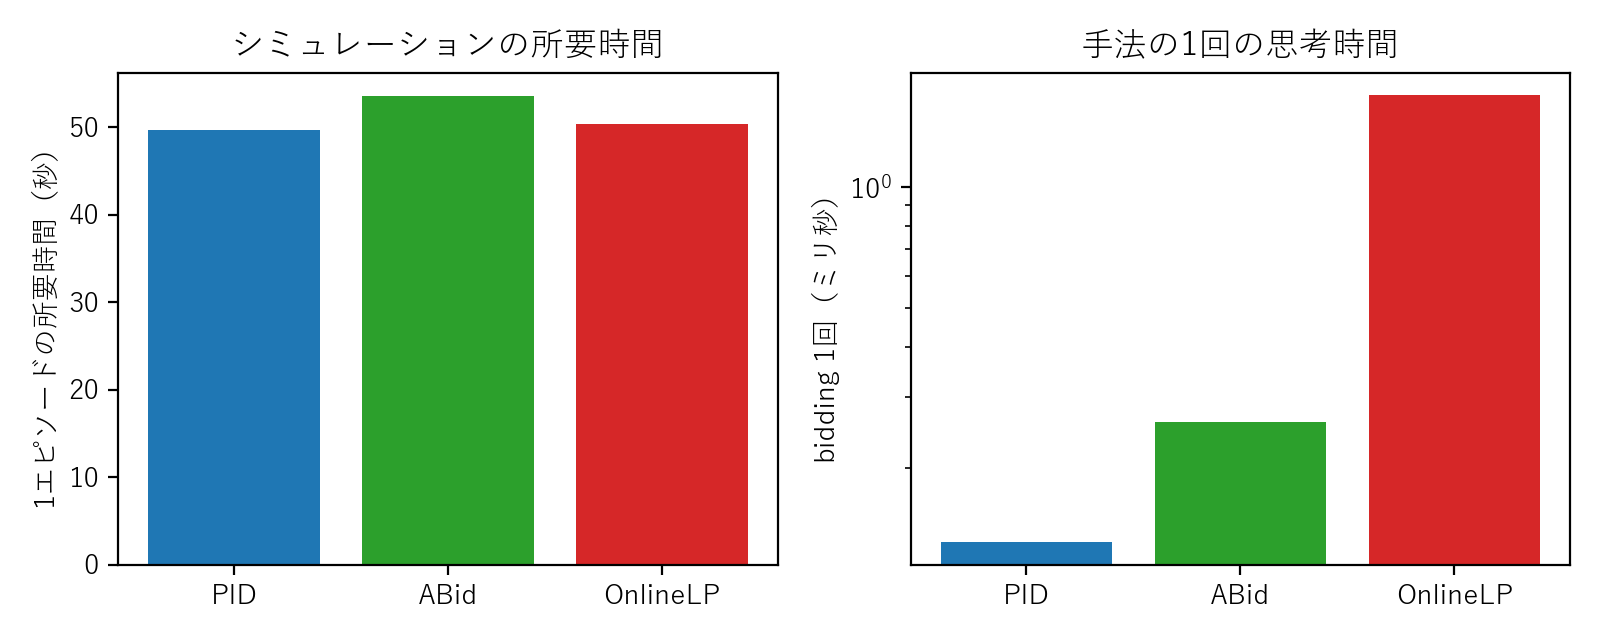
\includegraphics[width=0.9\linewidth]{fig/fig_scale.png}
\caption{所要時間。左：1エピソードのシミュレーション，右：\texttt{bidding()}1回（対数軸）}
\label{fig:scale}
\end{figure}

\textbf{再現性}　同じ設定の再実行で，\texttt{episodes}表の全列が全エピソードで完全に一致した（報酬・scoreの差は0.0）。

\textbf{3手法の比較}　表\ref{tab:cmp}と図\ref{fig:scores}のとおり，Online LPのscore合計は，PIDの1.92倍，ABidの1.49倍で最大であった（論文の「Online LPが最良」と同じ向き）。
なお，論文の図10（目視の概算）ではPIDはAbidの2〜3.5倍，Online LPは6〜7倍であり，本結果（PID 0.78倍，Online LP 1.49倍）とは，PIDとAbidの順序と倍率が一致しない（原因は未確認）。
セル単位でOnline LPがPIDを上回った割合は0.77，ABidを上回った割合は0.69，PIDがABidを上回った割合は0.42であった。
6カテゴリごと，4エピソードごとの合計は，すべてOnline LPが最大であった。
プレイヤー以外の47社の平均スコアは，手法によらず21.3〜21.4でほぼ同じであった。

\begin{table}[H]
\centering
\caption{既定設定の3手法（48位置×4エピソード，192セル）}
\label{tab:cmp}
\footnotesize
\begin{tabularx}{\linewidth}{@{}Xrrr@{}}
\toprule
 & ABid & PID & Online LP \\
\midrule
score合計（÷20000） & 0.165 & 0.128 & 0.246 \\
ABidを1.0とした値 & 1.00 & 0.78 & 1.49 \\
平均報酬（ペナルティ前） & 25.8 & 24.4 & 28.7 \\
ペナルティが掛かったセルの割合 & 0.85 & 0.82 & 0.39 \\
予算消化率の平均 & 0.93 & 0.99 & 0.75 \\
最終ティックより前に落札が止まった割合 & 0.81 & 0.56 & 0.41 \\
順位の中央値 & 32 & 35 & 18 \\
\bottomrule
\end{tabularx}
\end{table}

\begin{figure}[H]
\centering
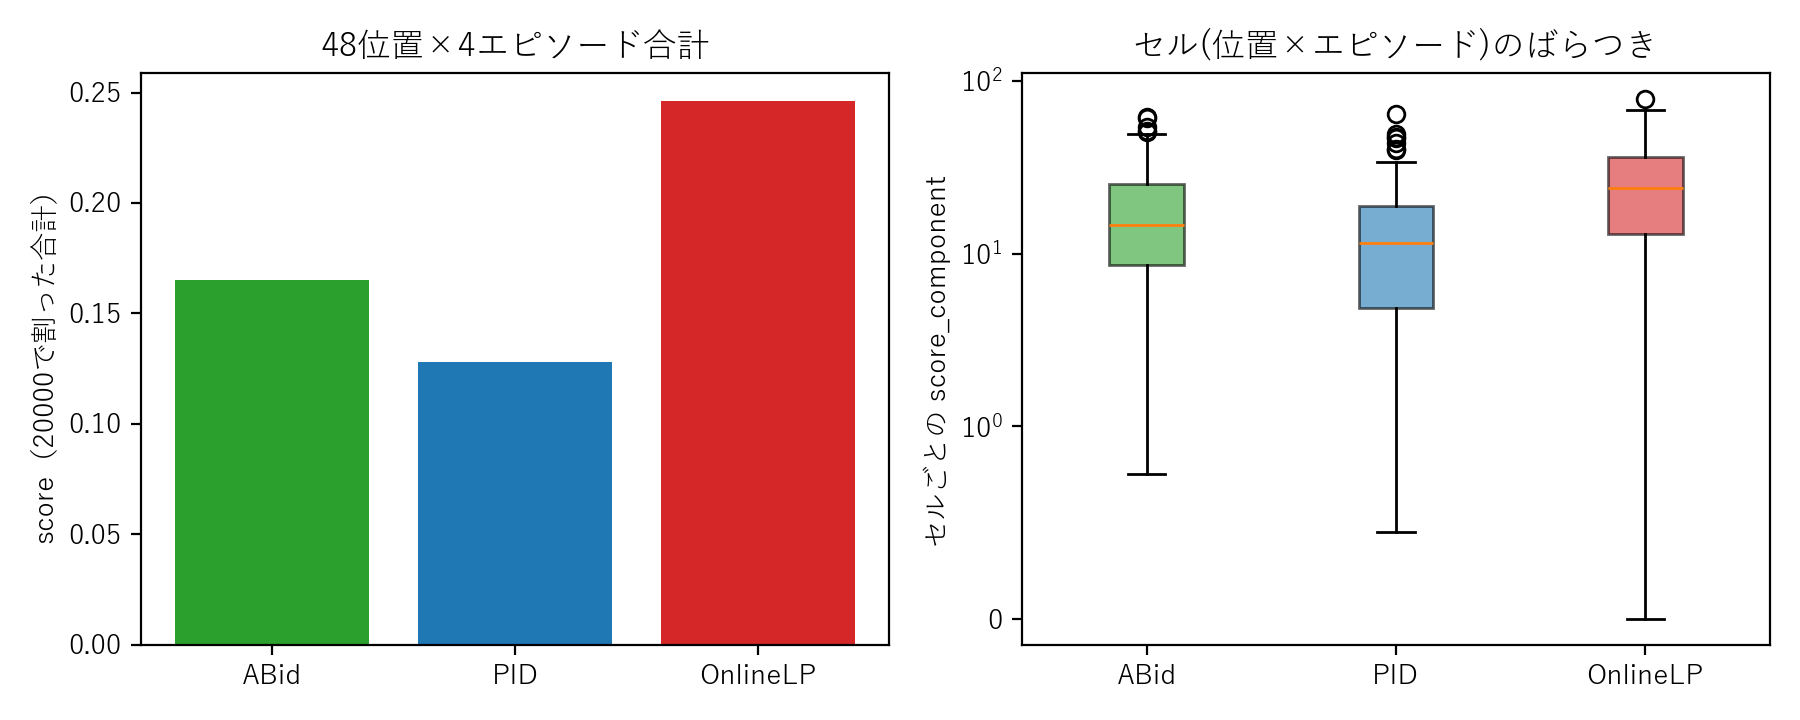
\includegraphics[width=\linewidth]{fig/fig_scores.png}
\caption{3手法のスコア。左：合計，右：セルごとの分布（symlog軸）}
\label{fig:scores}
\end{figure}

図\ref{fig:alpha}は，実効入札係数$\alpha$（入札額の和÷価値の和）などの時系列である。
PIDはティック0の$\alpha$が15で（他47社の中央値は68），落札数が0から立ち上がるのはティック7ごろ以降であった。
ABidはティック0〜20の$\alpha$が約115で，ティック23以降の中央値は0であった。
Online LPは全ティックで70〜89に収まり，他47社の中央値に近かった。


\textbf{パラメータ掃引}　図\ref{fig:sweeps}のとおり，振った範囲で最良点が既定値だったのは，Online LPの2つのパラメータだけであった。
既定値に対する最良点の比は，PIDで1.02〜1.18（\texttt{up\_factor}を1.2から1.1にすると1.18），ABidで1.39（\texttt{bid\_scale}を1から0.5にすると），
Online LPで1.00であった。ABidは入札倍率を0.25にすると0.45倍，4にすると0.14倍に落ちた。
同じ6位置で，既定のOnline LPは23.4，PIDの最良点は18.2，ABidの最良点は17.0であった。


\textbf{特徴量}　\texttt{episodes}（1,028行），\texttt{ticks}（49,344行），\texttt{agents}（49,344行）の全数値列に，NaN・無限大はなかった。

以上より，実験の前に決めた達成条件（REP001.md）をすべて満たし，探索の目的は\textbf{達成}した。

% ============================================================
\section{結果から生まれた問い}\label{sec:e-question}
% ============================================================

この環境で，ルールベース3手法は，広告主の位置を変えても完走し，Online LPのスコアが最大であった。
Online LPは，ペナルティが掛かったセルの割合が小さく（0.39），同時にペナルティ前の平均報酬も最大であった（28.7）。
PIDとABidは，既定値より良くなる設定があった（最大1.39倍）が，その最良点でも，既定のOnline LPには届かなかった。
1回の評価は，約150〜215秒・約2.5GBであり，手法の計算時間はコンペの制限に対して十分に小さかった。

まだ確かめていないが，Online LPの優位は，CPA制約を守ること（ペナルティが小さいこと）による部分が大きいと考えられる。
一方で，PIDの序盤の落札の遅れ（初期$\alpha$が低い）や，ABidの予算切れの早さが，PIDとABidの成績を下げている可能性もある。
また，Online LPは早見表を使うので，早見表の作られた条件が評価の環境と近いことが，成績に効いている可能性がある（確認していない）。
この環境での手法間の差を，ペナルティ前の報酬と，ペナルティ係数のどちらがどれだけ説明するのかを知りたい。

\end{document}
